\chapter{Missions complémentaires}
\label{chap:troisiemechapitre}

\section{Développeur au sein du projet MATRIX}

\subsection{Contexte du projet}

En plus de ma mission principale (participer aux développement de PPIL).
J'ai travaillé sur le projet transverse MATRIX interne à Sopra Steria de la CNAM Métier.
Nous avons formé une équipe de 6 stagiaires, et nous nous sommes réparti différents rôles (CP(1), RF(1), RT(1), BA(2), SB(2)).
Mon rôle pour ce projet est celui de SB (développeur).
Le temps alloué pour ce projet est d'une demi journée par semaine.
 
\subsection{Un besoin}

L'objectif premier est la recherche de compétence pour la création d’une équipe.

Ce projet a été mis en place suite à la demande de mon manager de projet, qui au sein du pôle a certains besoins que les outils existant ne satisfont pas. Nous avons donc eu un démarche de compréhension du besoin du client :
Les manager de projet ont besoin de rechercher des compétences parmi les collaborateurs du pôle dans l’optique de créer des équipes de développeur ou de chercher une personne compétente dans une technologie particulière.

\subsubsection{L'importance d'étudier les outils existant}

Pour réaliser cette tâche de recherche de collaborateurs répondant à certaines compétences, Les manager de projets ont des outils / processus déjà existant tel que :

Le premier outil utilisé au niveau du pôle CNAM métier étant un fichier Excel qui répertorie les compétences des collaborateurs. Cette solution pose des difficultés principalement au niveau de la maintenabilité des informations à jour.

La deuxième solution qui s'offre aux manager de projet est, dans l'intranet du groupe (tout Sopra Steria), une section de recherche d'expert en fonction d'une compétence. Cet outil ne répertorie qu'une partie des collaborateurs (les experts dans un domaine), et la localisation de ceux-ci n'est pas à jour.

\begin{figure}[!h]
\centering
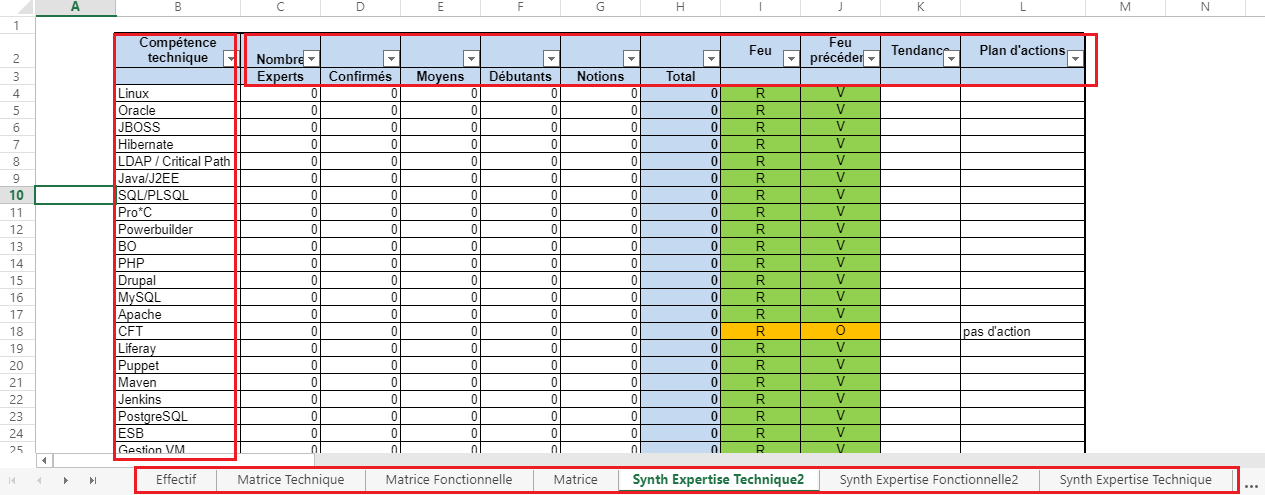
\includegraphics[width=1\textwidth]{images/MATRIX-excel.png}
\caption{MATRIX : Template du document Excel qui recense les collaborateurs en fonction de leurs compétences}
\end{figure}

Il est important d'analyser ce document car c'est celui-ci qui dans la pratique est utilisé par les manager de projet. Pour la conception de notre application, il est important de prendre en compte la façon dont les information sont agencés dans ce fichier Excel.

Au vu des outils et processus cité ci-dessus, on voit bien que l'application MATRIX a bien sa place au sein du pôle CNAM métier et qu'elle serait un réel atout pour les manager de projets.

\subsection{Concevoir une application, notre démarche}

Lors de la conception de l'application, nous nous sommes retrouvés face à diverses problématiques. 

Par exemple, lorsque nous nous sommes demandés comment seront géré la liste des compétences en BDD : qui et comment seront ajouté les compétences, 

nous nous sommes retrouvés face à plusieurs questions : est-ce qu'un utilisateur peut ajouter lui même une fonctionnalité ? Ou est-ce qu'elle sont déterminées en base de données ? Si elles sont déterminées en base de données comment en ajouter une nouvelle ? faut il faire des demandes administrateur ? Est-ce que les détails de la compétence (image, version ?) seront transmises avec ?

Toutes ces questions, nous avons pu y répondre grâce à :
- l'étude des outils existants (document Excel)
- différents points avec le client
- priorité et faisabilité des fonctionnalités en un temps déterminé

Nous avons choisi de :
ne pas prendre en compte les différentes versions des technologies. (grâce au document excel)
de ne mas passer par l'admin pour ajouter une technologie. (grâce aux entretiens avec le client)
qu'il y aura une liste par défaut des technologies en base de données.(grâce au document excel)
l'ajout d'une base de donnée sera géré dans le lot 2.

\subsubsection{Classer les fonctionnalités par priorité : Lot 1 et Lot 2}
Concernant les droits d’accès pour chacun des 3 profils (collaborateurs, administrateur projet et administrateur général) il a été décidé de voir ça au lot 2 et de se concentrer pendant le lot 1 sur l’objectif principal. Petit flou sur les droits d’administrateur projet à la création d’un projet car cela fait partie du lot 1 (Le détail du lot 1 sera détaillé par la suite).


\subsection{Choix des technologies}

Nous avons été libre de choisir les technologies : 
- Java Spring 
- JHipster 
- JavaScript

Spring est un socle pour le développement d'applications très répandu en entreprises. Il représente un réel avantage en nous fournissant de nombreuses fonctionnalités qui peuvent être utilisés de plusieurs manières : ceci nou laisse le choix au développeur d'utiliser la solution qui correspond le plus à nos besoins.
Spring est ainsi un des frameworks les plus répandus dans le monde Java et dispose d'une grande popularité.

JHipster fournit des outils pour générer un projet avec côté serveur, une pile Java (à l'aide de Spring Boot) et côté client un frontal Web adaptatif (avec Angular et Bootstrap).
JHipster nous permet d'atteindre nos objectif, avec plus de productivité, de l'outillage et de la qualité.

JavaScript, le grand incontournable des pages web interactives. JHipster étant lui même construit en parti en Angular (framework JavaScript).

\subsection{Avancement des travaux}
\subsubsection{Compte rendu 22/05}

Bilan :

Lecture des SFG existant, nous avons fait le point sur certaines précision de
- l’objectif premier à savoir la recherche de compétence pour la création d’une équipe
- les droits d’accès en fonction des types de profils
- discussion et choix des fonctionnalités à destination du lot 1
- Qui va faire la liste des compétences en BDD ?
- récupération des docs existant On a besoin de ce qui à déjà été fait sur excel -> demander l’accès au fichier (filtres, profils etc…)
- Les CU sont listés avant les maquettes ? Lister les maquettes correspondantes aux CU dans la même partie ?
- faire des maquettes 

Objectif semaine prochaine :

En règle générale, il faut corriger les scénarios nominaux (syntaxe parfois floues ou fausses) et rajouter des scénarios exceptionnels et alternatifs.

\subsubsection{Compte rendu 30/05}

Bilan :

- Retour sur les questions du CR1
- Les maquettes pas prioritaires pour le moment
- Rédaction des CU
- proposition d'utiliser Jhipster

Objectif semaine prochaine :

- Terminer les sfd avant la semaine prochaine (retour des SFG pour le 12)
- Maquettes avant le 24 juin // et commencer les dev en parallèle 
- faire le planning
- démo d’installation de JHipster
- Se renseigner sur les règles de rédaction des SFD

\subsubsection{Compte rendu 6/06}

Bilan :

- Installation JHispter
- Installation IDE
- Mis en place du git lab. 

Objectif semaine prochaine :

- Modification des CU
- (Lot 2) Finition des CU sur un Projet (Ajout, suppression, etc..)

\subsubsection{Compte rendu 13/06 }

Bilan :

- Début de rédaction des STD (Template)
- Schéma de la base de donnée
- Maquette pour les SFD

Objectif semaine prochaine :

- Valider la base de donnée auprès d'un expert
- Finir les SFD

\subsection{Mise en place des SFG **}

spécifications fonctionnelles SFG
    - pour le projet entier
    - pour le lot 1
spécifications techniques (STD = spécification techniques détaillées)

\subsection{Mise en place des STD **}

\subsection{Les maquettes **}

Nous avons réalisé des maquettes du projet MATRIX en nous basant sur celles déjà existantes. Ci-dessous voici une des 7 maquettes.

\begin{figure}[!h]
\centering
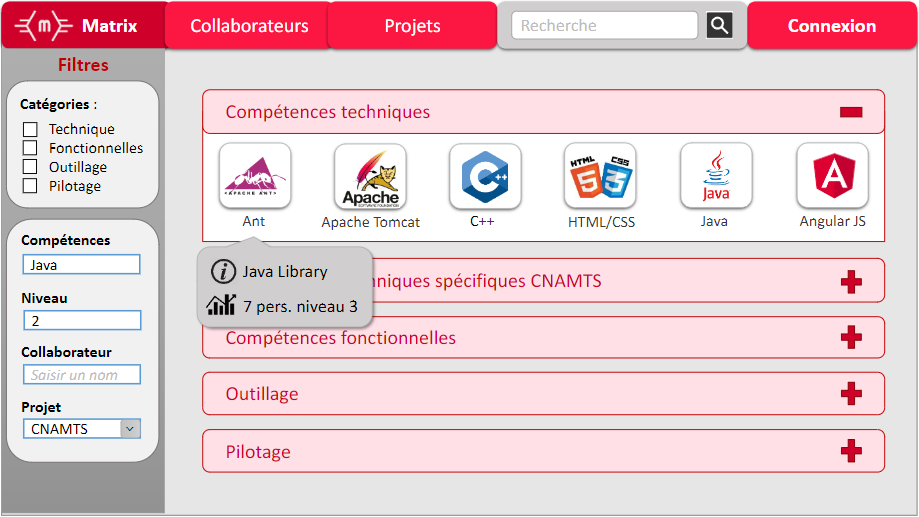
\includegraphics[width=1\textwidth]{images/matrix-maquette.png}
\caption{MATRIX : Maquette de recherche par compétence}
\end{figure}

\begin{figure}[!h]
\centering
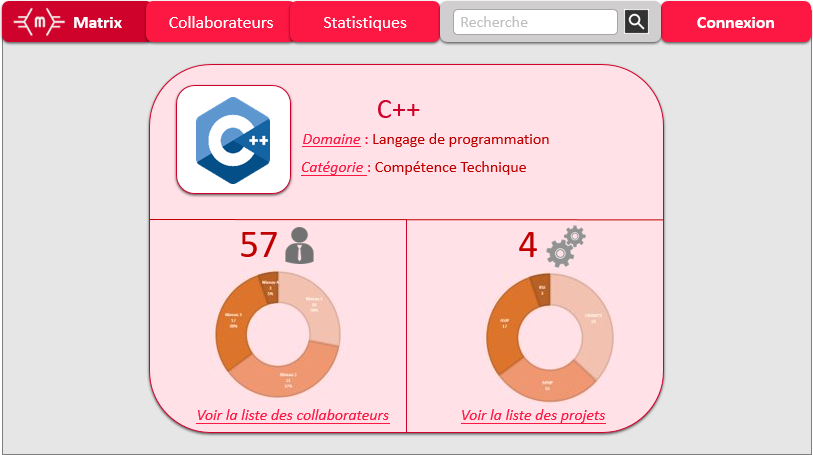
\includegraphics[width=1\textwidth]{images/matrix-maquette-competence.png}
\caption{MATRIX : Maquette détail d'une compétence}
\end{figure}

\subsection{La BDD **}

\begin{figure}[!h]
\centering
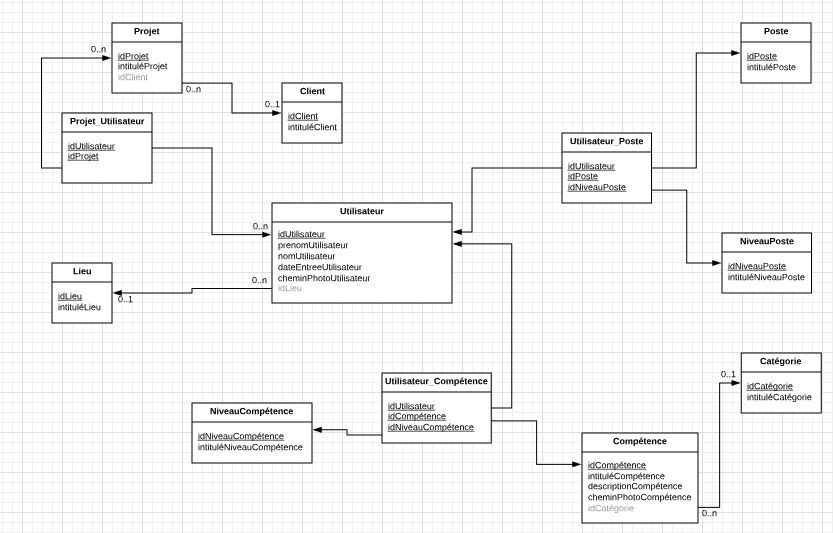
\includegraphics[width=1\textwidth]{images/matrix-bdd.png}
\caption{MATRIX : MCD}
\end{figure}

\subsection{Installation de l’environnement **}

Git Intellij Gitlab

\section{Interview et Présentation du métier de Business Analyste en vidéo}

Sopra Steria a proposé à tous les stagiaires de l'agence des volontaires pour réaliser une vidéo de présentation du métier de BA. Cette vidéo est destiné à présenter le métier aux nouveaux arrivants sur le pôle.
Je me suis porté volontaire avec deux autres stagiaires pour réaliser cette mission. 
Nous avons pris l'initiative de réaliser des interview filmé de 3 collaborateurs, des BA de niveau 3. 
En parallèle nous avons crée une animation sur l'outil Powtoon. Puis nous avons réalisé un montage vidéo en fusionnant les interview et l'animation Powtoon.
Cette vidéo a été présenté à tous les acteurs du pole Cnam Métier (nombre de personnes), la vidéo a été très appréciée.

Cette mission a été l'occasion de découvrir et d'échanger avec des collaborateurs expérimentés et de découvrir ce métier.

\begin{figure}[!h]
\centering

\includegraphics[width=0.5\textwidth]{images/presBA.png}
\caption{Sopra Steria : Présentation du métier de BA}
\end{figure}
%%% Local Variables: 
%%% mode: latex
%%% TeX-master: "isae-report-template"
%%% End: 